%#!platex tls.tex
\chapter{執筆}

\begin{abstract}
\laTEX は WYSIWYG 形式のプログラムではありませんので,原稿をタイプセット
して出力ファイルを閲覧するという方式となっております.そこで原稿を
タイプセットするために何らかのテキストエディタか統合環境を用いる事
になると思います.この章ではそれらテキストエディタや統合環境の基本的な
使い方を紹介します.筆者の主な環境が \Prog{Vine Linux} と \Prog{Mac OS X}
であるため,解説もそれに依存したものになっておりますので,適宜
ご自分の環境に沿うように読み替えてください.
\end{abstract}

\section{GNU Emacs}

伝統的な\Z{テキストエディタ}として \Prog{vi} や \Prog{ed} などが
ありますが,\LaTeX を使う上で便利な環境になると思われるのは,
やはり \Prog{GNU Emacs} (本冊子では単に Emacs と表記します) だと思われま
す.いくら時代遅れだと人に言われても,Emacs 使いは廃れる事はないでしょう.
Emacs はその機能を \Z{Emacs Lisp} という拡張マクロを用いる事で自由にカス
タマイズできる仕様になっています.\Prog{Windows} であれば \Prog{Meadow},
Mac OS であれば \Prog{Carbon Emacs} なるものを使うと良いでしょう.

インストール方法などに関してはお使いの環境によって千差万別だと
思われますので,適当にウェブの情報を参照してください\footnote{%
\Prog{Vine Linux} であれば \Z{root 権限}で
\type{apt-get install emacs color-mate}のようにします.}.

Emacs では \keytop{Ctrl} や \keytop{Alt} キーを組み合わせて様々な操作を
行なう事が可能です.

\keytop{Ctrl}-\keytop{h} \keytop{t} として,
まずはチュートリアルを実際に読み進める事をお薦めします.

\section{スペルチェック}

欧文を執筆している時に単語のスペルミス等を機械的にチェックして貰えると有
り難いものです.\Person{Pace}{Willisson}らによる\Prog{Ispell}等を使うこ
とにより対話的にスペルチェックを行なう事ができます.

Emacsからも\keytop{Alt}-\keytop{X} \type{ispell} 
としてIspellを呼び出す事ができます.コンソールからは
\type{ispell -t file.tex}として,\LaTeX の原稿の時は \copt{-t} オプショ
ンを付与します.

実行するとユーザと対話的に辞書ファイルに登録されていない単語をどうするか,
問い合わせを行ないます.
このとき,ユーザ側からは次の操作を指定できます.

\begin{description}
 \item[\keytop{R}] (それ以降の)ある単語を手動入力の修正候補で置き換えます.
 \item[\keytop{Space}] ある単語をその時だけ正しいものとします.
 \item[\keytop{A}] ある単語を今回のみ正しいものとします.
 \item[\keytop{I}] ある単語を正しいものとし,単語を辞書に登録します.
 \item[\keytop{U}] \keytop{I}の場合に加えて小文字の場合の単語も登録します.
 \item[\keytop{0--n}] 表示されている修正候補で置き換えます.
 \item[\keytop{L}] 単語を辞書ファイルから検索します.
 \item[\keytop{X}] Ispellを終了しカーソルを現在の位置に設定します.
 \item[\keytop{Q}] すぐにIspellを終了します.
 \item[\keytop{?}] ヘルプを表示します.
\end{description}

\begin{Prob}
 もしも\Prog{curl}, \Prog{ispell} をコンソール上から実行でき
 るのであれば,次のようにispellを実行してみて下さい.
\begin{InTerm}
 \type{curl -O http://tex.dante.jp/ok/de.tex; ispell -t de.tex}
\end{InTerm}
上記のプログラムがなければ,ご自分で適当な英文まじりにファイルを用意して,
Ispellと対話してみてください.
\end{Prob}

\section{Ya\TeX}

Emacs 上で動作する Emacs Lisp で書かれた \laTEX 支援環境として
\Prog[YaTeX]{Ya\TeX} があります.類似品として\Prog{AUC\TeX}も存在します
が,筆者の好みと利便性の面から言って\prog{Ya\TeX}をお勧めします.
Emacs と同様にインストール方法は適当に調べてください\footnote{%
\Prog{Vine Linux}では\type{sudo apt-get install yatex}で終わりです.}.

%\begin{append}
% この辺にYa\TeX の使い方についてのチュートリアルを記述する.
%\end{append}

\begin{Prob}
 
Ya\TeX の全ての機能を把握するまでにはある程度の時間を必要とします.
ここではチュートリアル程度の内容に留めた説明をします.

まず,適当なファイル \fl{yatest.tex} を作成してください.
Emacs のウィンドウ下部には次のような表示があるものと思います.

\dosh{-u:-- yatest.tex All (1,0)(やてふ Fill)}

\end{Prob}


\section{Make}
小規模な文書,例えば\Z{端物}やレポートなどであれば,Emacs と YaTeX を
組み合わせれば十分な執筆環境を得る事が出来ます.しかし,\Z{書籍}のように
大規模な文書になると原稿が複数ファイルに分かれていたり,画像やその他の
要素が絡んでくる場合があります.そのような時は一つの方法として,
伝統的に \Z{Makefile} を作成し,\Prog{Make} する事が考えられます.

(GNU) Make は再コンパイル支援ツールです.複数のファイルの依存関係を調べ
て,ソースファイルのコンパイルを楽にします.このツールを \LaTeX のタイプ
セットにも使用することが出来ます.

まずは簡単な例を一つ.
\begin{Makefile}
F=input
all: $F.dvi
$F.dvi: $F.tex
	 platex $F && platex $F
\end{Makefile}

変数 \str{$F} に入力ファイル \fl{input.tex} の \suf{tex} という拡張子を
取り除いたファイル名を書きます.次に標準のターゲット \str{all} を
\str{$F.dvi} (\fl{input.dvi}に展開される) に指定します.これにより%$
\fl{input.dvi} の作成を最終目標とします.次に \str{$F.dvi} の依存ファイ
ルを指定します.この場合は簡単に \str{$F.tex} とします.次に行は,行頭に
タブ文字を書き,続けて \str{$F.tex} から \str{$F.dvi} を生成するために必
要な作業を記述します.ここでは \Prog{platex} プログラムを 2 回ほど走らせ
ることになります.

\subsection{\fl{Makefile} の実際の表記 }

\fl{Makefile} 中では便利な省略表記が使われます.頻繁に使われるものは次の三つです.

\begin{description}
 \item[\str{$<}]
    入力ファイル名
 \item[\str{$*}]
    入力ファイル名から拡張子を取り除いたもの
 \item[\str{$@}]
    出力ファイル名
\end{description}%$

標準的な \fl{Makefile} は,次の三つの部分に分かれています.
\begin{description}
   \item 各種変数の宣言
   \item 一般的な依存関係とファイル生成規則
   \item 実ファイルの依存関係
\end{description}
各種変数の宣言とは次のようにコマンドやコマンドラインオプションなどを保存
します.
\begin{Makefile}
TEX=platex
PDFOPT=-p a4 -r 2400 -V 4 -o $@
F=test
\end{Makefile}
\TeX には主となる TeX エンジン,PDFOPT には Dvipdfmx のコマンドラインオ
プション,F には原稿となる \TeX ファイル名(拡張子なし)を記述します.変
数を使用するときは \$(TEX) 等として,先頭にドルを追加し,全体をパーレンで
くくります.

次に一般的な依存関係を記述します.普通, \fl{file.tex} から PDF を生成するには
\begin{InTerm}
\type{platex file.tex}
\type{dvipdfmx file.dvi}
\end{InTerm}
とするので,依存関係に関わる処理は次のように記述します.
\begin{Makefile}
.tex.dvi:
	$(TEX) $<
.dvi.pdf:
	dvipdfmx $(PDFOPT) $<
\end{Makefile}
次に実ファイルの依存関係を記述します.まずは標準のターゲット,最終的に作
成したい(とは限らないが)ファイルを次のように指定します.
\begin{Makefile}
all: $F.pdf
\end{Makefile}
このようにして,実際の依存関係を明記します.
\begin{Makefile}
$F.pdf: $F.dvi
$F.dvi: $F.tex
\end{Makefile}
しかし,実はこのままではうまく行きません.Make に対して,新規に次の拡張
子を登録します.
\begin{InText}
.SUFFIXES: .tex .dvi .pdf
\end{InText}
この \Suf{SUFFIXES} は \str{$*} 等で必要になりますので,ファイルの先頭に
でも記述すると良いでしょう.%$

このようにして,次のようなファイル \Fl{Makefile} が完成します.
\begin{Makefile}
.SUFFIXES: .tex .dvi .pdf
TEX=platex
PDFOPT=-p a4 -r 2400 -V 4 -o $@
F=test

.tex.dvi:
	$(TEX) $<
.dvi.pdf:
	dvipdfmx $(PDFOPT) $<

all:	$F.pdf

$F.pdf: $F.dvi
$F.dvi: $F.tex
\end{Makefile}
実際に \fl{test.tex} を次のように作成し Make コマンドを引数なしで実行し
てください.
\begin{InText}
\documentclass{jarticle}
\begin{document}
test
\end{document}
\end{InText}
これを\type{make}とすると
\begin{InTerm}
 \type{platex test.tex}
 \type{dvipdfmx -p a4 -r 2400 -V 4 -o test.pdf}
\end{InTerm}
を実行したのと等価になります.ためしにもう一度
\begin{InTerm}
 \type{make}
\end{InTerm}
として,
\begin{OutTerm}
 make: Nothing to be done for `all'.
\end{OutTerm}
と表示されれば,きちんと依存関係が記述されていることになります.さらに
\begin{InTerm}
\type{touch test.tex}
\end{InTerm}
と実行して,ファイルのタイムスタンプを変更し
\begin{InTerm}
 \type{make}
\end{InTerm}
と実行するともう一度 \pLaTeX と \dvipdfmx が実行され \fl{test.pdf} が生成されます.

まぁ,普段は次のような \fl{Makefile} を用意するだけで実は良かったりします.
\begin{Makefile}
.SUFFIXES: .tex .dvi .aux .log .toc .lof .lot .pdf .ps
F=gs20050501
TEX=platex

all:	$F.dvi

pdf:	$F.pdf
ps:	$F.ps
dvi:	$F.dvi

$F.dvi: $F.tex
$F.pdf: $F.dvi
$F.ps:  $F.dvi

.dvi.ps:
	dvips -Ppdf -o $@ $<
.dvi.pdf:
	dvipdfmx $<
clean:
	rm -f *~ $F.dvi $F.aux $F.lof $F.toc $F.lot $F.log $F.pdf $F.ps
\end{Makefile}
いやはや,実は \JBibTeX も使っているという人は以下のように変更すれば良い
でしょう.%$
\begin{Makefile}
.SUFFIXES: .tex .dvi .aux .log .toc .lof .lot .pdf .ps .bbl .bib .blg
F=gs20050501
TEX=platex

all:	$F.dvi
pdf:	$F.pdf
dvi:	$F.dvi
bbl:	$F.bbl
ps:	$F.ps

$F.dvi: $F.tex $F.bbl
$F.pdf: $F.dvi
$F.ps:	$F.dvi
$F.bbl: $F.bib
$F.aux: $F.tex

.dvi.ps:
	dvips -Ppdf -o $@ $*
.dvi.pdf:
	dvipdfmx $*
.bib.bbl:
	platex $*; jbibtex -kanji=sjis $*; platex $*
.tex.aux:
	$(TEX) $*

clean:
	rm -f *~ $F.dvi $F.aux $F.lof $F.toc $F.lot $F.log \
		$F.pdf $F.ps $F.bbl $F.blg
\end{Makefile}
さらに索引とか用語集とか,いろいろある人はまぁ,適当に.折角なのでプレ
ビューと印刷も簡単にできるようにしておきましょう.依存関係とか適当に書い
て終わりです.


\subsection{もっと高度な例}
\begin{Makefile}
.SUFFIXES: .tex .dvi .aux .log .toc .lof .lot .pdf .ps .bbl .bib .blg .lol .cls .sty .eps .eepic .plt .out .obj .title

F=	m1201234
SRC=	title.pl rmlgbm.map
CLS=	funthesis.cls
setting=gsset.sty
abst=	00abst.tex

TEX=	 platex
#DVIPDF= dvipdfmx -f rmlgbm.map -p a4 -V 4
DVIPDF=	dvipdfmx -p a4 -V 4
BIBTEX=	jbibtex
RM=	rm -f
AUTOMAKE= make
MKDIR=	mkdir -p

#your favorite line printer name
#LPNAME=	printername
LPNAME= 	192.168.11.2

# for Mac OS X with EasyPackage/Mac pTeX 
XDVI=  open -a Mxdvi.app
PDFVIEWER=open
DVIPS= dvips -t a4

# for Unix/Linux/Solaris/BSD/...
#XDVI= xdvi
#PDFVIEWER=acroread

# for Windows
#XDVI= dviout 
#PDFVIEWER=iexplore

all: $F.pdf README 

pdf:   $F.pdf
ps:    $F.ps
dvi:   $F.dvi
bbl:   $F.bbl
2up:   $(F)up.ps
title: $F.title

view:  $F.dvi
	$(XDVI) $<
viewpdf: $F.pdf
	$(PDFVIEWER) $<
check: $F.pdf
	pdfinfo $<
	pdffonts $<
README:        $(setting)
	cat $< | grep -e "^%%" | sed -e "s/^%%//;" > README
today: $F.pdf
	cp $< $F-`date +%Y-%m-%d-%H-%M`.pdf
#img:
#      cd img && $(AUTOMAKE)

$F.dvi:        $F.tex
$F.pdf:        $F.dvi
$F.ps: $F.dvi
$(F)up.ps: $F.ps
$F.bbl: $F.bib
$F.aux: $F.tex
$F.title: $(abst)

.dvi.pdf:
	$(DVIPDF) $*
$(F)up.ps: $F.ps
	psnup -2 $< $@
.dvi.ps:
	$(DVIPS) -o $@ $*
.bib.bbl:
	$(TEX) $*; $(BIBTEX) $*; $(TEX) $*
.tex.dvi:
	$(TEX) $<
	(while egrep "may have changed" $*.log; \
		do $(TEX) $<; done)
.tex.aux:
	$(TEX) $*
.tex.title:
	echo "cat $(setting) $F.tex | ./title.pl > $F.title"

fast:
	$(TEX) $F; $(TEX) $F
faster:
	$(TEX) $F;

clean:
	$(RM) *~ $F.dvi $F.aux $F.lof $F.toc $F.lot $F.log \
		$F.ps $F.bbl $F.blg $F.lol $F.out
	$(RM) *.dvi *.aux *.log *.toc *.blg *.bbl *.lof *.lot

tar: $F.tex title README $(SRC) $(CLS) 
	$(MKDIR) $(F)src/img
	cp $F.tex $F.title Makefile README $(SRC) $(CLS) $(F)src/
	cp img/* $(F)src/img/
	tar czf $(F)src.tgz $(F)src/
	rm -fr $(F)src

# Gnuplot の場合
SRC := $(wildcard img/*.plt)
obj := $(patsubst %.plt,%.eps,$(SRC))
pdfobj := $(patsubst %.plt,%.pdf,$(SRC))
# Tgif の場合
TGIF := $(wildcard img/*.obj)
tgifobj := $(patsubst %.obj,%.eps,$(TGIF))
tgifpdfobj := $(patsubst %.obj,%.pdf,$(TGIF))

img: $(pdfobj) $(tgifpdfobj)

.plt.eps:
	gnuplot $<
	mv `basename $@` img/
.obj.eps:
	tgif -print -eps -color $<
.eps.pdf:
	epstopdf $<
	pdfinfo $@|grep -e 'Page size:'|sed -e 's/x//; s/Page size:/\%\%BoundingBox: 0 0 /; s/pts//;'>$*.bb

$(obj): %.eps: %.plt
$(pdfobj): %.pdf: %.eps

$(tgifobj): %.eps: %.obj
$(tgifpdfobj): %.pdf: %.eps

cleanimg:
	echo "rm -f *.bb *.eps *.pdf"
\end{Makefile}

%\section{latexmk}
%
%とかは既に初級編で解説済み.


\section{WinShell}

WinShellはWindows用の\LaTeX 執筆支援環境です.
初期設定は\TeX\ Wiki\footnote{http://oku.edu.mie-u.ac.jp/~okumura/texwiki/?WinShell}等を参照してください.

\begin{center}
 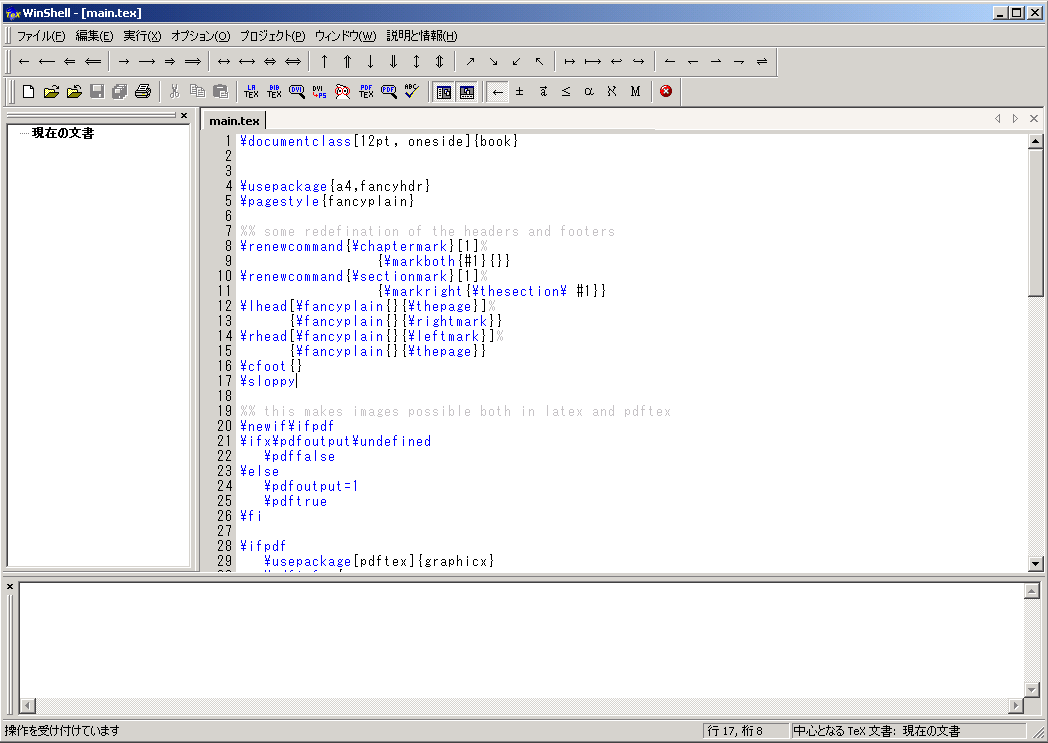
\includegraphics[scale=.4]{images/WinShell}
\end{center}

\begin{append}
 この辺にWinShellに関する使い方の解説を追加する.
\end{append}

\section{Easy\TeX}

Easy\TeX もWindows用の\LaTeX 執筆支援環境です.作製者が
日本人なので,インタフェースのすべてが日本語です.

\begin{center}
 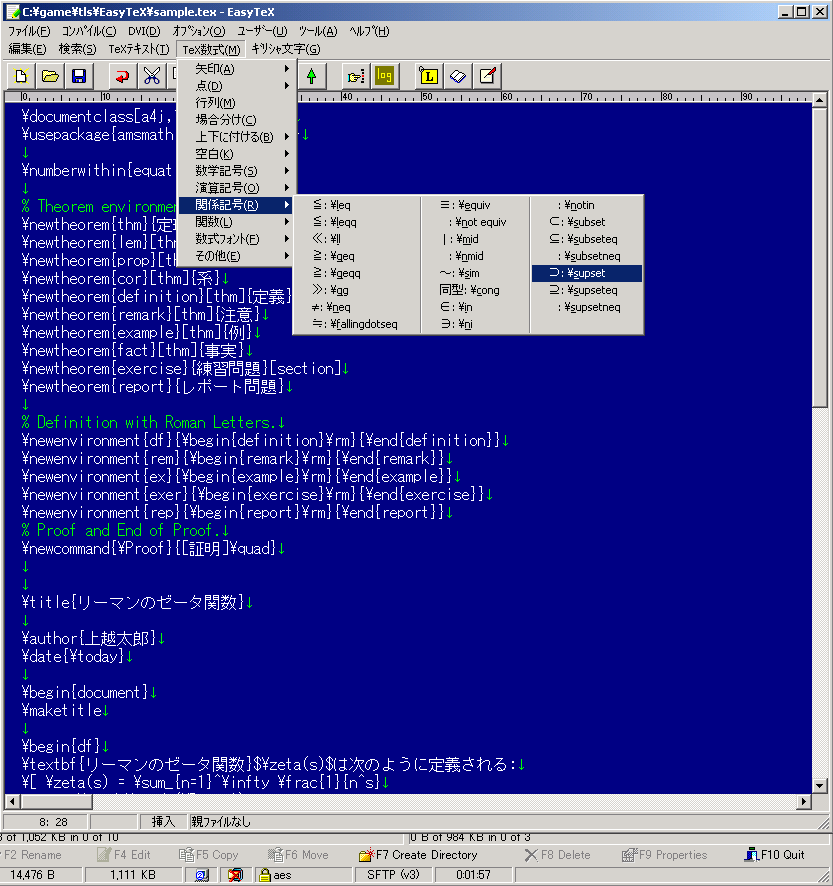
\includegraphics[scale=.4]{images/EasyTeX}
\end{center}

\begin{append}
 この辺にEasy\TeX に関する使い方の解説を追加する. 
\end{append}

\section{TeXShop}

\Prog{Mac OS X}に話しが限られますが,\laTEX の統合環境として,
\Prog[TeXShop]{\TeX Shop}があります.

因に \Prog[XeTeX]{\XeTeX} と \prog{\TeX Shop} を組み合わせると \Prog{Mac
OS X} の \Z{ATSUI} と呼ばれるフォント機構に直接アクセスでき,且つ PDF ファ
イルのプレビューもできるため,大変便利です.

Emacs キーバインディングでのキー操作が出来ますので,Emacs使いでも
使いやすいと思います.

\begin{figure}[htbp]
 \begin{center}
 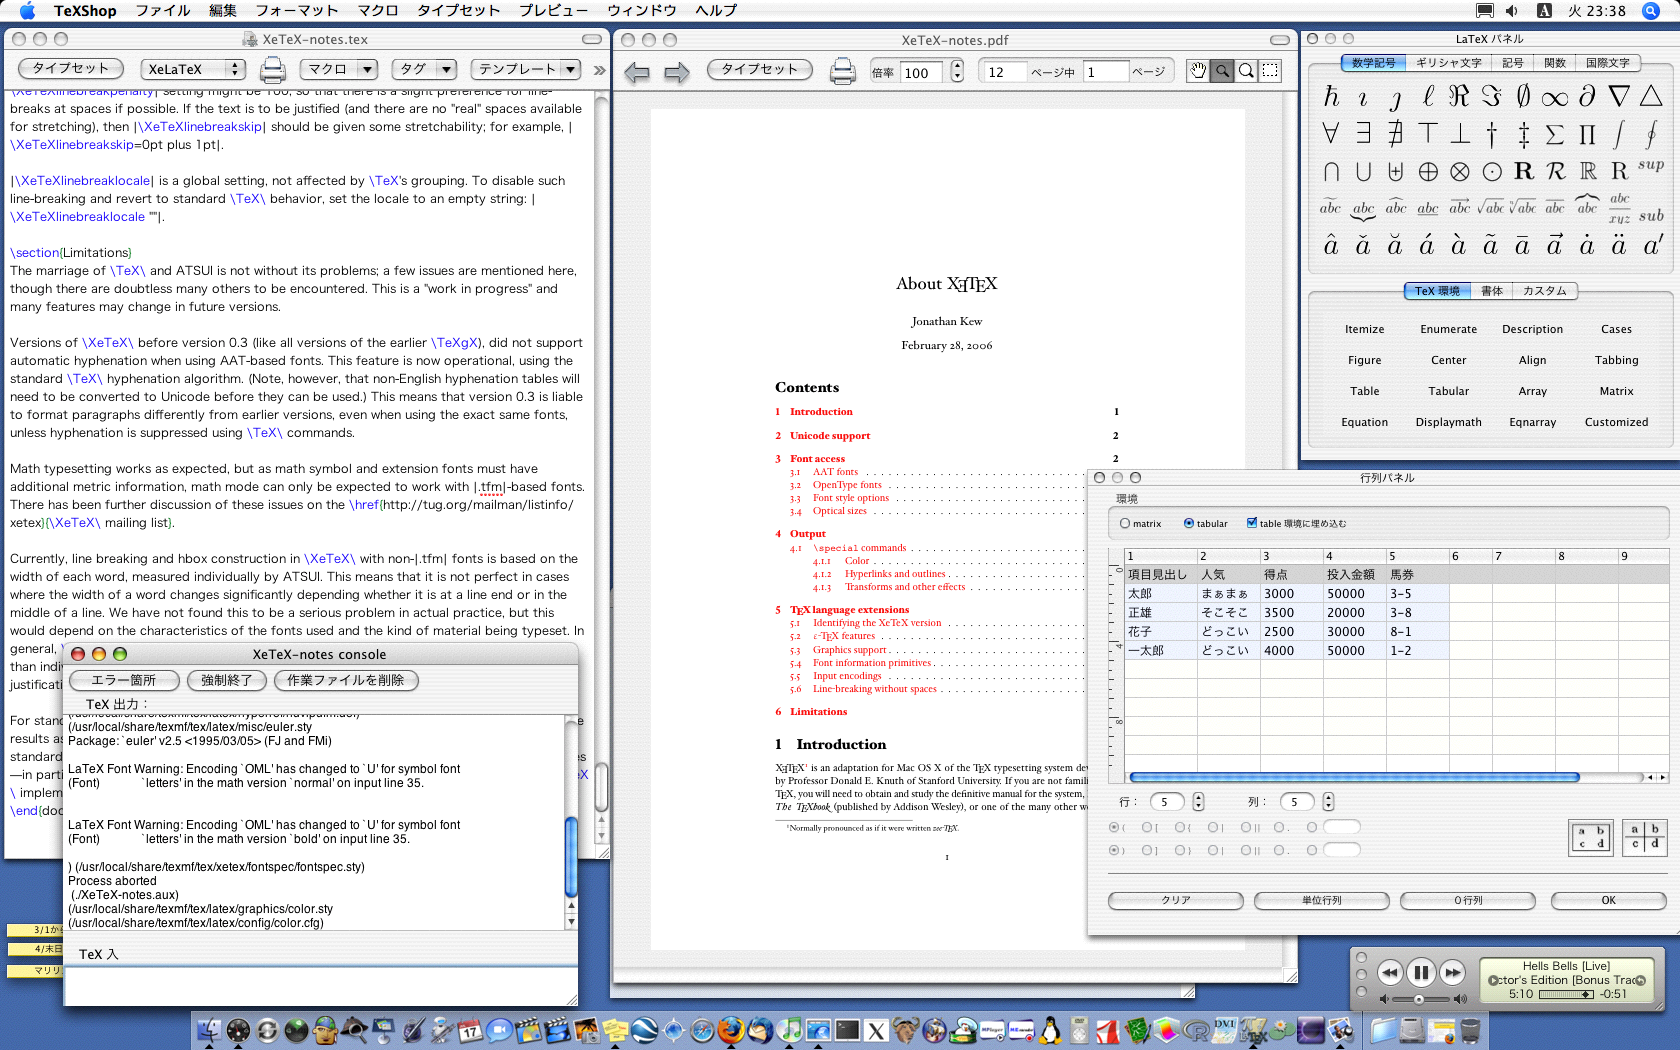
\includegraphics[width=\linewidth]{images/TeXShop01}
 \caption[\TeX Shop の起動画面]
 {起動画面です.左上が原稿ウィンドウ,左下が,タイプセットログを表示するコ
 ンソールウィンドウ,中央がPDFのプレビューウィンドウ.右上が \LaTeX パ
 ネルと呼ばれるもので,数学記号,ギリシャ文字,記号,関数,国際文字,
 \TeX 環境,書体指定コマンドなどをクリックで入力できる.右下は行列パネ
 ル.これで簡単な表や行列を簡単に作成できます.
 これくらいの作業を行おうと思えば20インチ以上のシネマディスプレイが欲
 しくなる所です.}
 \end{center}
\end{figure} 

\begin{figure}[htbp]
 \begin{center}
 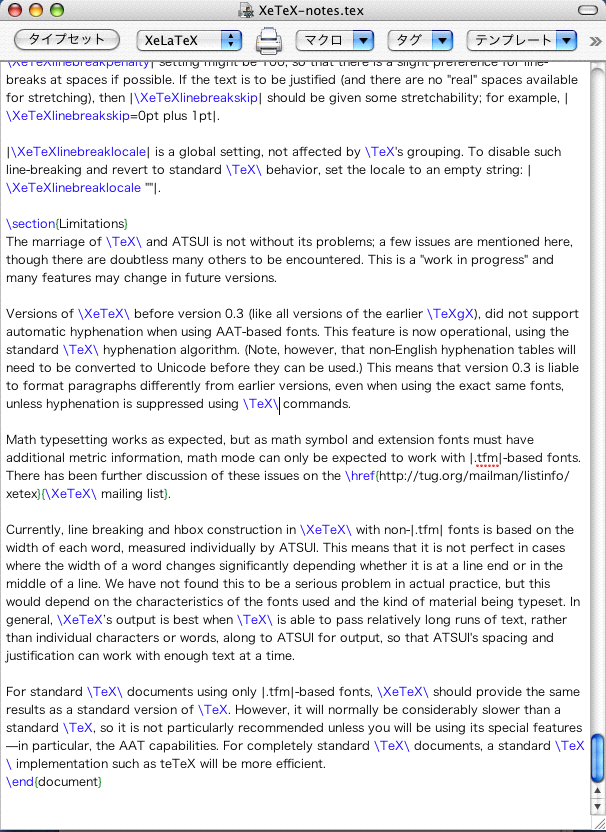
\includegraphics[scale=.4]{images/TeXShop02} 
 \caption[\TeX shop の原稿ウィンドウ]{%
  原稿ウィンドウです.\TeX コマンド等は強調表示されます.ウィンドウ上部の
  「タイプセット」ボタンを押す事によりタイプセットが実行できます.「タ
  イプセット」ボタン右側のセレクトボタンから\prog{mendex} や \prog{\JBibTeX} 等の他の
  プログラムも選択できます.「マクロ」「タグ」「テンプレート」から\TeX
  マクロや\LaTeX 環境をクリックする事で入力できます.}
 \end{center}
\end{figure}

\begin{figure}[htbp]
 \begin{center}
 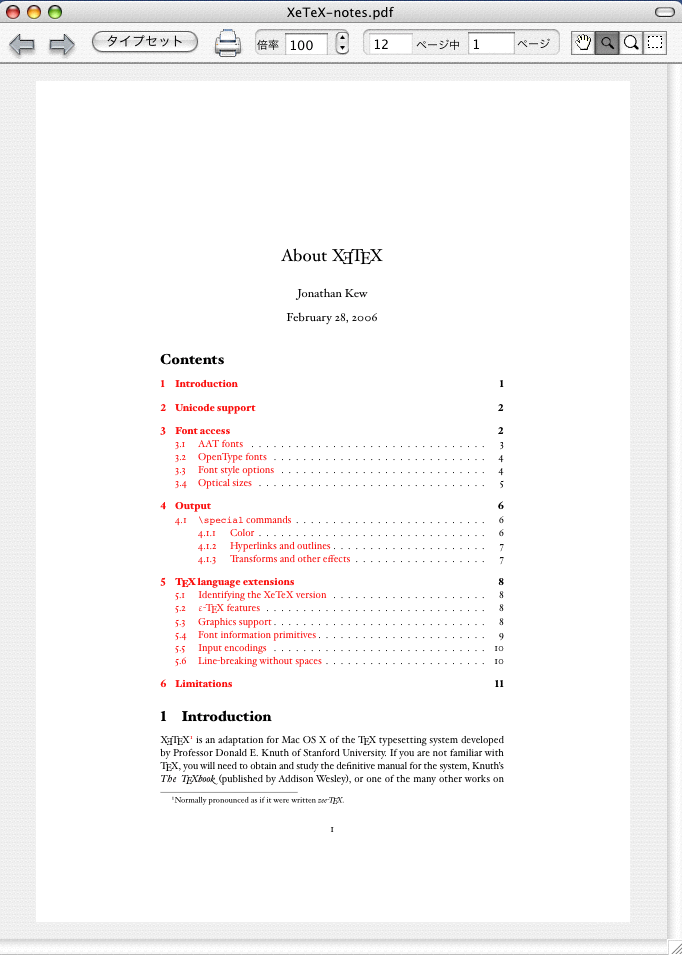
\includegraphics[scale=.4]{images/TeXShop03} 
 \caption[\TeX Shop のプレビューウィンドウ]{
  プレビューウィンドウです.ウィンドウ丈夫に操作ボタンが幾つかあります.
  通常のPDF文書と同じように,ページ送り,印刷,表示倍率指定,拡大ツール
  等があります.}
 \end{center}
\end{figure}

\begin{figure}[htpb]
 \begin{center}
 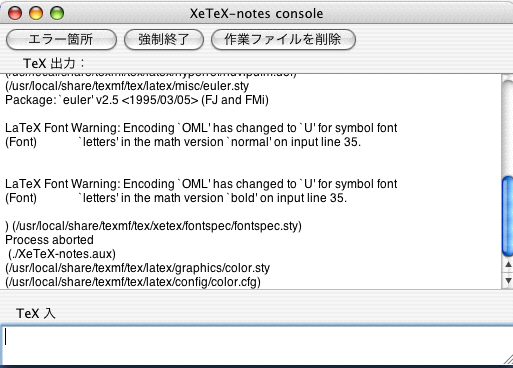
\includegraphics[scale=.4]{images/TeXShop04} 
 \caption[\TeX Shop のログウィンドウ]{
  タイプセットのログウィンドウです.ここに \TeX の処理過程とエラー・警
  告などが表示されます.「エラー箇所」ボタンを押す事でエラーが発生して
  いる行に移動します.「\TeX 入」のテキストフィールドに文章を入力する事
  で,インタラクティブな操作を行う事ができます.}
 \end{center}
\end{figure}

\begin{figure}[htbp]
 \begin{center}
 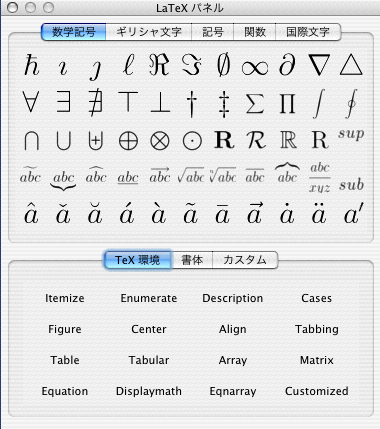
\includegraphics[scale=.4]{images/TeXShop05} 
  \caption[\TeX Shop の\LaTeX パネル]{
  記号類や環境等をマウスで簡単に入力するための\LaTeX パネルです.若干
  \Y{amssymb}, \Y{amsmath} パッケージを必要とする記号類も含まれているか
  もしれません.}
 \end{center}
\end{figure}

\begin{figure}[htbp]
 \begin{center}
 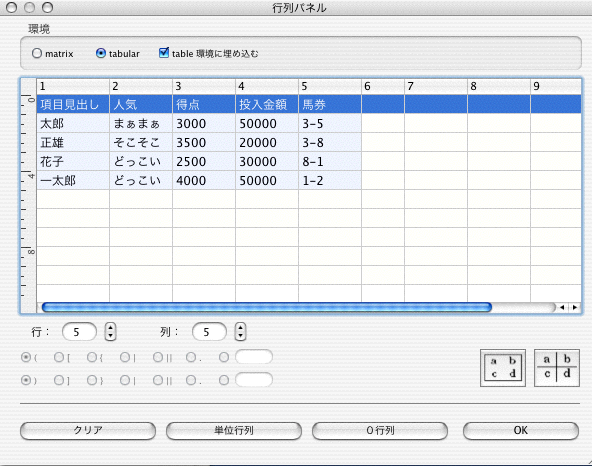
\includegraphics[scale=.4]{images/TeXShop06} 
  \caption[\TeX Shop の行列パネル]{
  行列パネルです.\E{matrix}環境か\E{tabular}環境の何れかを選択します.
  罫線に関する処理もある程度行なう事が出来ます.\Z{単位行列}や\Z{零行列}の
  入力も簡単にできるようにボタンが用意されています.}
 \end{center}
\end{figure}

\begin{figure}[htbp]
 \begin{center}
 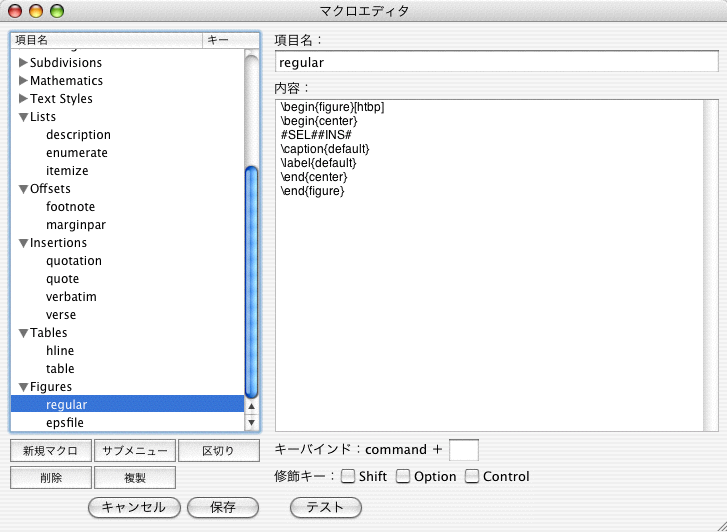
\includegraphics[scale=.4]{images/TeXShop07} 
 \caption[\TeX Shop のマクロエディタウィンドウ]{
  マクロエディタウィンドウです.自作のマクロを新規に追加し,良く使う記
  述を登録する事が出来ます.勿論,登録済のマクロの編集も可能です.ショー
  トカットキーの登録も出来るようになっています.}
 \end{center}
\end{figure}

\begin{figure}[htbp]
 \begin{center}
 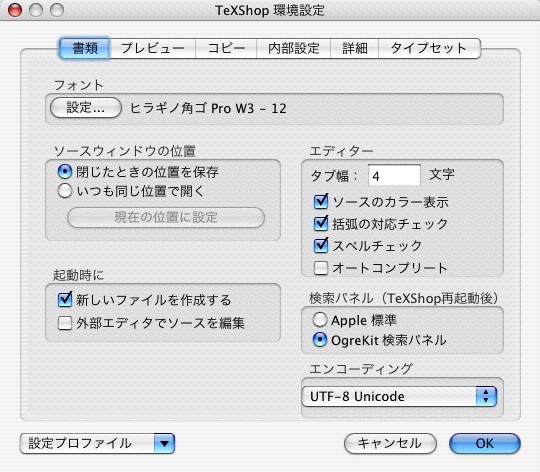
\includegraphics[scale=.4]{images/TeXShop08} 
 \caption[\TeX Shop の環境設定ウィンドウ]{
  \TeX Shop 環境設定ウィンドウです.「書類」「プレビュー」「コピー」
  「内部設定」「詳細」「タイプセット」タブが上部に存在します.フォント
  は好みに合わせて設定してください.「設定プロファイル」というセレクト
  ボタンがありますので,こちらから適切なプロフィアルを選択してみて下さ
  い.}
 \end{center}
\end{figure}



\section{その他}


\begin{append}
 この辺に何かしらの追加すべき事項を記述する.
\end{append}
